\documentclass[conference]{IEEEtran}
\IEEEoverridecommandlockouts

\usepackage{cite}
\usepackage{amsmath,amssymb,amsfonts}
\usepackage{algorithmic}
\usepackage{graphicx}
\usepackage{textcomp}
\usepackage{xcolor}
\usepackage{tikz}
\usepackage{threeparttable} % Supports footnotes inside tables
\usepackage{graphicx} % Add this to your preamble
\usepackage{tabularx} % Add this to your preamble
\usepackage{comment}
%\usepackage{float}
%\usepackage[skip=5pt]{caption} % Add this in the preamble
\setlength{\textfloatsep}{8pt} 

%\usetikzlibrary{shapes, arrows, positioning}

\bibliographystyle{IEEEtran}

\begin{document}

%\title{Fuzzy Logic-Based Maximum Power Point Tracking for PV Battery Chargers}

\title{Fuzzy Logic-Based MPPT with Advanced Buck Converter Modeling for PV Battery Chargers}

\author{\IEEEauthorblockN{Mehmet Gök, Kemal Ozanoglu, and Günhan Dündar}
\IEEEauthorblockA{\small{Department of Electrical and Electronics Engineering, Bogazici University}}
}
\maketitle

\begin{abstract}
This paper presents the modeling of a Fuzzy Logic Controller (FLC) for Maximum Power Point Tracking (MPPT) in photovoltaic (PV) battery charging systems, incorporating an advanced buck converter model.
The proposed system enhances MPPT performance by leveraging fuzzy logic to handle nonlinearities and uncertainties while improving power conversion efficiency through a more detailed switching model of the buck converter.
Previous works on MPPT have incorporated buck converters; however, they primarily relied on simplified models that did not accurately capture power losses. This work introduces a Simulink-based MPPT implementation featuring a synchronous switching buck converter model. This approach provides a more accurate representation of power losses, including switching losses and non-overlapping losses, leading to improved power conversion modelling.
The system is validated through comprehensive Simulink simulations under dynamically changing solar irradiation conditions, including efficiency analysis, charge current evaluation, and transient response assessment to ensure accurate performance validation. 
The results highlight the benefits of integrating a refined buck converter model with fuzzy logic-based MPPT, establishing a more reliable framework for future research and development in similar applications.
\end{abstract}

\begin{IEEEkeywords}
Fuzzy Logic Control, Maximum Power Point Tracking (MPPT), Photovoltaic (PV) Systems, Buck Converter, Battery Charging, Energy Efficiency
\end{IEEEkeywords}



\section{Introduction}
The increasing demand for renewable energy sources has led to the widespread adoption of photovoltaic (PV) systems for power generation \cite{pvbook}. As the global focus shifts toward sustainable energy solutions, PV technology continues to evolve, offering improved efficiency and cost-effectiveness. However, a major challenge in PV energy harvesting is maximizing power extraction under varying environmental conditions. This challenge is addressed through Maximum Power Point Tracking (MPPT) algorithms, which continuously adjust the system to operate at the optimal power point \cite{mpptpavia}. Traditional MPPT methods, such as Perturb and Observe (P\&O) and Incremental Conductance (IC), are commonly used but often suffer from inefficiencies due to their sensitivity to rapid fluctuations in solar irradiation. Fuzzy Logic Control (FLC) has emerged as a promising alternative due to its ability to handle nonlinearities and uncertainties, making it well-suited for MPPT applications in PV systems \cite{zadeh1965fuzzy}.

Previous works have extensively explored the use of Simulink for modeling PV energy conversion systems \cite{simulink2024}. Simulink provides a versatile simulation environment that allows for rapid prototyping, system-level analysis, and the ability to incorporate complex control algorithms with minimal computational overhead. Researchers have leveraged Simulink to study the behavior of MPPT algorithms, power converters, and overall system dynamics, demonstrating its effectiveness in evaluating the performance of PV systems.

Recent studies on modeling PV buck converters with MPPT in Simulink typically employ simplified switching models for the DC-DCFuzzy Logic-Based MPPT with Advanced Buck converter topology \cite{recent1robles2017fuzzy, recent2iqbal2016msu, recent3sathya2013modelling,recent4,recent5}. These models often rely on asynchronous buck converter designs that use a single switch and a diode. While such configurations offer simplicity and ease of implementation, they tend to result in suboptimal performance, reduced efficiency, and increased losses due to non-ideal switching behavior. The lack of detailed switch modeling limits the accuracy of these simulations, failing to capture the true dynamics of power conversion in practical implementations. To address these limitations, this work presents an enhanced buck converter model in Simulink that incorporates a more realistic switching representation incorporating synchronous switching, resulting in improved efficiency and more accurate MPPT performance.

%dummy paragraf
%The remainder of this paper is structured as follows: Section II details the system design and modeling, covering the PV model, buck converter, and fuzzy logic-based MPPT controller. Section III presents the performance analysis of the proposed buck converter model. Finally, Section IV concludes the paper.

\begin{figure}[ht]
\centering
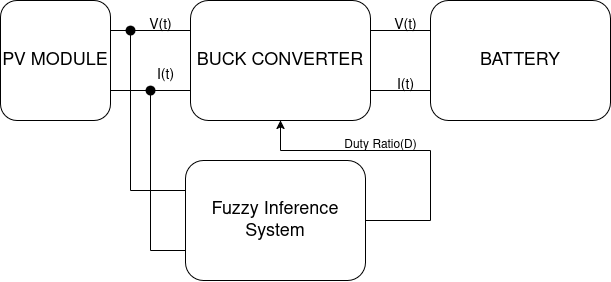
\includegraphics[width=0.8\columnwidth]{smacd_pvbucl.drawio.png}
\caption{Simplified schematic of the advanced buck converter used in PV battery charging systems.}
\label{fig1:buck_design}
\end{figure}


\begin{figure*}[h]
    \centering
    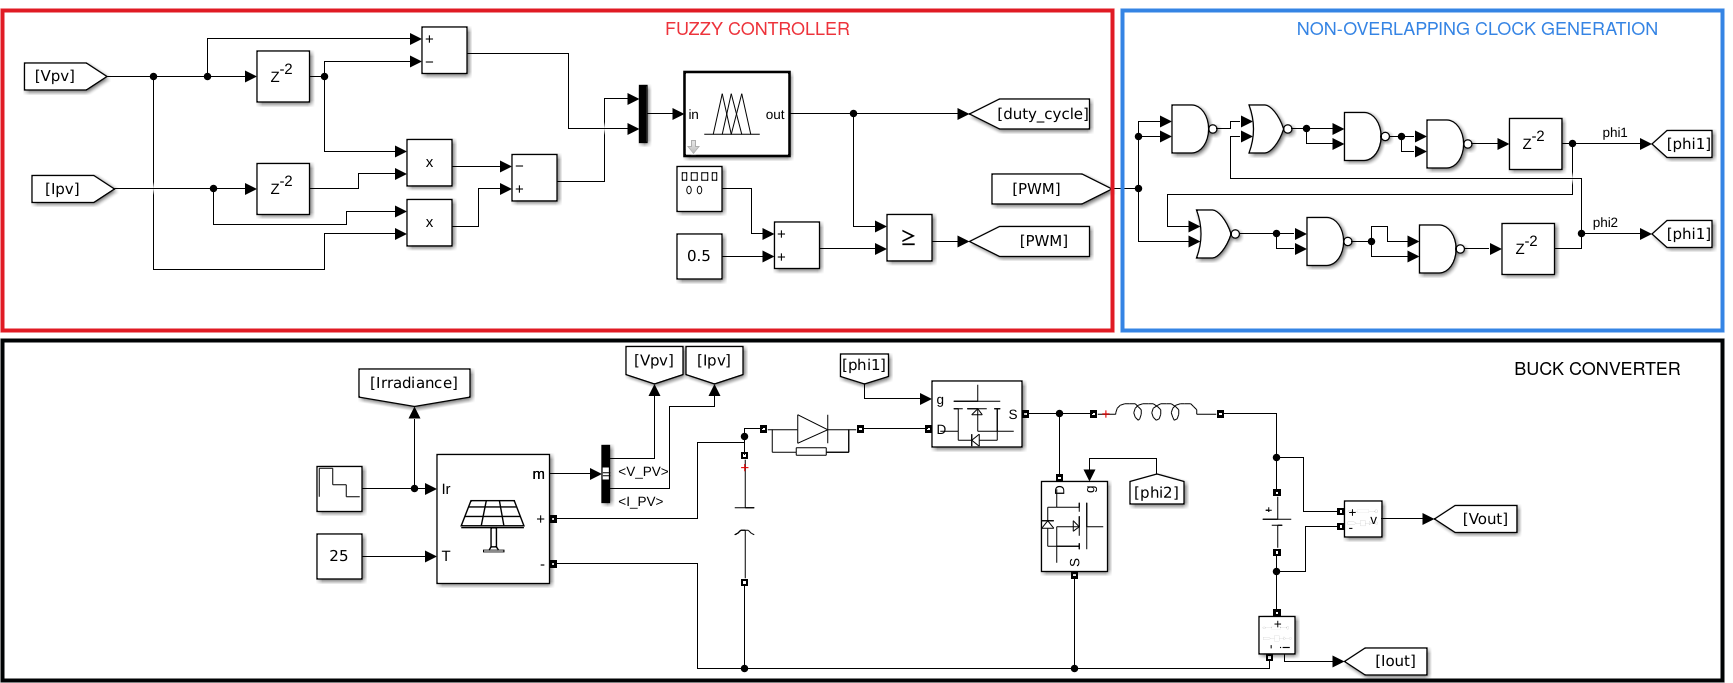
\includegraphics[width=0.8\textwidth]{matlab_smacd.drawio.png} 
    \caption{Complete Simulink model of the proposed Fuzzy Logic-based MPPT system. The model includes the photovoltaic panel, buck converter, and fuzzy logic controller to simulate real-world operating conditions.}    
    \label{fullsetup}
\end{figure*}



\section{System Design and Modelling}

%\subsection{Solar Panel and Buck Converter}
The solar panel is chosen for our work is model 6MN6A280 from Ablytek with non-ideal characteristics, such as varying input conditions. The buck converter steps down the voltage from the PV panel to the level required by the battery while maintaining high efficiency. The design of the buck converter is optimized to operate at its maximum efficiency point, ensuring minimal power loss during the conversion process.

    

\subsection{Buck Converter Performance}
The buck converter is a critical component of the PV battery charging system. It steps down the voltage from the PV panel to the level required by the battery while maintaining high efficiency. The design of the buck converter is optimized to operate at its maximum efficiency point, ensuring minimal power loss during the conversion process. To evaluate the performance of the buck converter, a DC voltage source is connected to the output to emulate the battery. The output current (\(I_{out}\)), PV efficiency, and converter efficiency are measured as a function of the duty cycle.
\vspace{\baselineskip}

\subsubsection{Output Current vs Duty Cycle}
The relationship between the output current (\(I_{out}\)) and the duty cycle is critical for understanding the behavior of the buck converter. As the duty cycle increases, the output current initially rises, reaching a maximum value at the optimal duty cycle. Beyond this point, further increases in the duty cycle lead to a decrease in output current due to non-ideal effects such as switching losses and inductor saturation, as given in Figure \ref{fig:duty_current}.

\begin{figure}[ht]
\centering
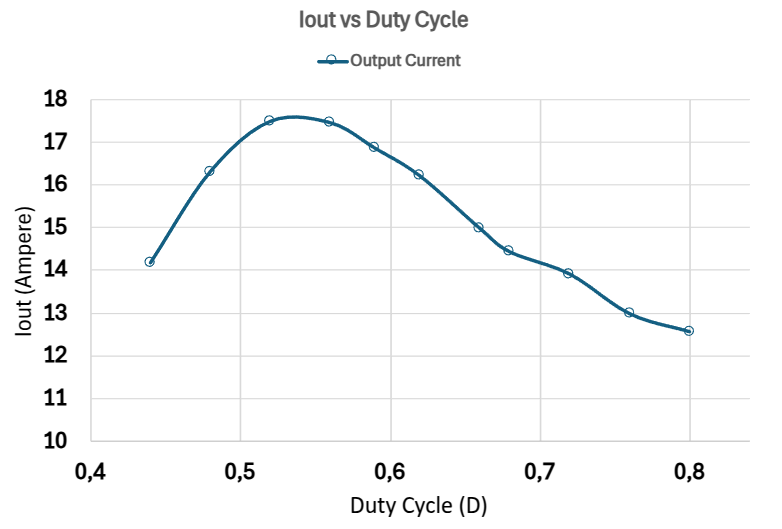
\includegraphics[width=0.8\columnwidth]{iotvsD.png}
\caption{Duty cycle versus output current for the buck converter. The peak output current occurs at the optimal duty cycle, indicating the maximum power point (MPP) of the PV panel.}
\label{fig:duty_current}
\end{figure}
\vspace{\baselineskip}

\subsubsection{PV Efficiency vs Duty Cycle}
The efficiency of the PV system is directly influenced by the duty cycle of the buck converter. At low duty cycles, the efficiency is suboptimal due to insufficient power transfer. As the duty cycle increases, the efficiency improves, reaching a maximum at the optimal duty cycle, as shown in Figure \ref{duty_pv_efficiency}. Beyond this point, efficiency decreases due to increased losses in the converter.

\begin{figure}[ht]
\centering
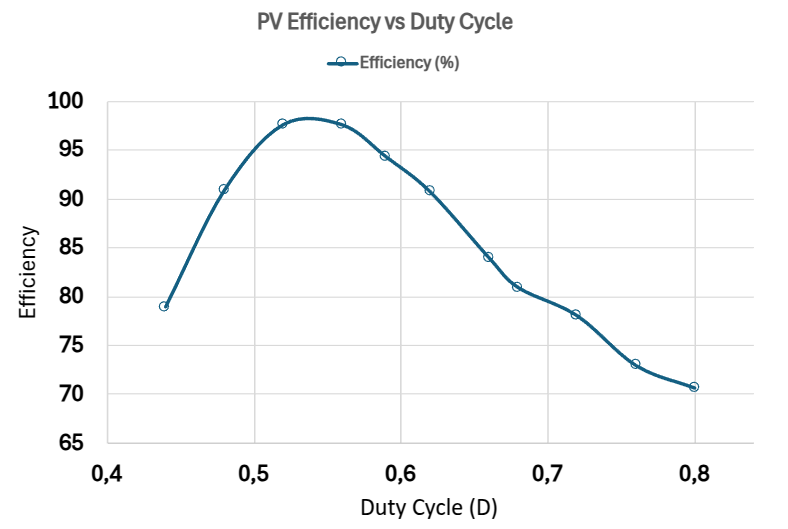
\includegraphics[width=0.8\columnwidth]{pveffvsD.png}
\caption{Duty cycle versus PV efficiency for the buck converter. The peak efficiency corresponds to the optimal duty cycle, ensuring maximum power transfer from the PV panel to the battery.}
\label{duty_pv_efficiency}
\end{figure}
\vspace{\baselineskip}

\subsubsection{Converter Efficiency vs Duty Cycle}
The efficiency of the buck converter itself is also a key performance metric. Converter efficiency is defined as the ratio of output power to input power. At low duty cycles, the converter efficiency is low due to high conduction losses. As the duty cycle increases, the efficiency improves, reaching a maximum at the optimal duty cycle, as given in Figure \ref{duty_converter_efficiency}. Beyond this point, switching losses and inductor core losses dominate, leading to a decrease in efficiency.

\begin{figure}[ht]
\centering
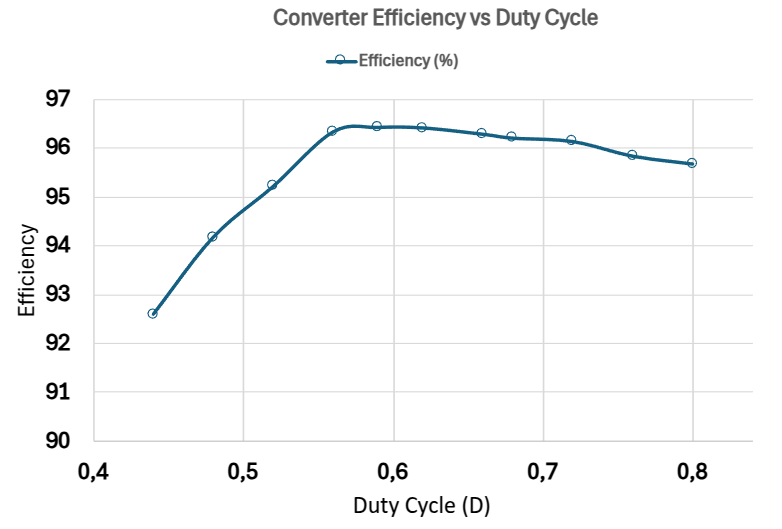
\includegraphics[width=0.8\columnwidth]{conveffvsD.png}
\caption{Duty cycle versus converter efficiency for the buck converter. The peak converter efficiency aligns with the optimal duty cycle, ensuring minimal power loss during the conversion process.}
\label{duty_converter_efficiency}
\end{figure}
\vspace{\baselineskip}
Hence according to above results maximizing PV efficiency will be enough for maximizing output current which is critical for battery charging applications.

\subsection{Fuzzy Inference}
The control loop model is critical for ensuring the system operates at the maximum power point (MPP). The Fuzzy Logic Controller (FLC) is designed to dynamically adjust the duty cycle of the buck converter to track the MPP. The FLC uses two input variables: the change in power (\(\Delta P\)) and the change in voltage (\(\Delta V\)). These inputs are defined as follows:

\begin{equation}
\Delta P = P(t) - P(t-1)
\end{equation}

\begin{equation}
\Delta V = V(t) - V(t-1)
\end{equation}

where:
\begin{itemize}
    \item \(P(t)\) is the instantaneous power at time \(t\),
    \item \(P(t-1)\) is the power at the previous time step,
    \item \(V(t)\) is the instantaneous voltage at time \(t\),
    \item \(V(t-1)\) is the voltage at the previous time step.
\end{itemize}
\vspace{\baselineskip}

\subsubsection{Fuzzy Logic Controller Design}
The FLC is designed to handle the nonlinear relationship between \(\Delta P\) and \(\Delta V\). The input variables are fuzzified using membership functions. The output is determined based on a 5x5 fuzzy rule table, given by Table \ref{tab:fuzzy_rules}, that maps the fuzzified inputs to the appropriate control action. These rules ensure that the FLC adjusts the duty cycle to move the operating point toward the MPP.
\vspace{\baselineskip}

\subsubsection{Membership Functions}
The membership functions for \(\Delta P\) and \(\Delta V\) are defined using three distinct shapes: triangular, S, and Z shapes. These functions map the crisp input values to fuzzy sets, such as \textit{Negative Large (NL)}, \textit{Negative Small (NS)}, \textit{Zero (Z)}, \textit{Positive Small (PS)}, and \textit{Positive Large (PL)}. The output membership function is similarly defined to represent the control action, as given by Figures \ref{fig5:membership_deltaP},  \ref{membership_deltaV}, and \ref{fig7:membership_output}. 

\begin{figure}[ht]
\centering
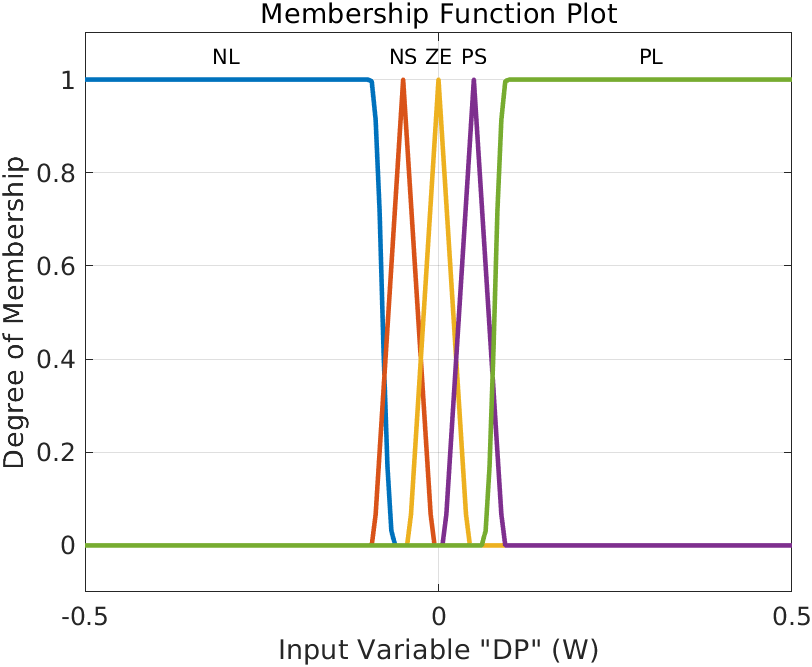
\includegraphics[width=0.8\columnwidth]{DP.png}
\caption{Membership functions for \(\Delta P\). The input is fuzzified into five linguistic variables: Negative Large (NL), Negative Small (NS), Zero (Z), Positive Small (PS), and Positive Large (PL).}
\label{fig5:membership_deltaP}
\end{figure}

\begin{figure}[ht]
\centering
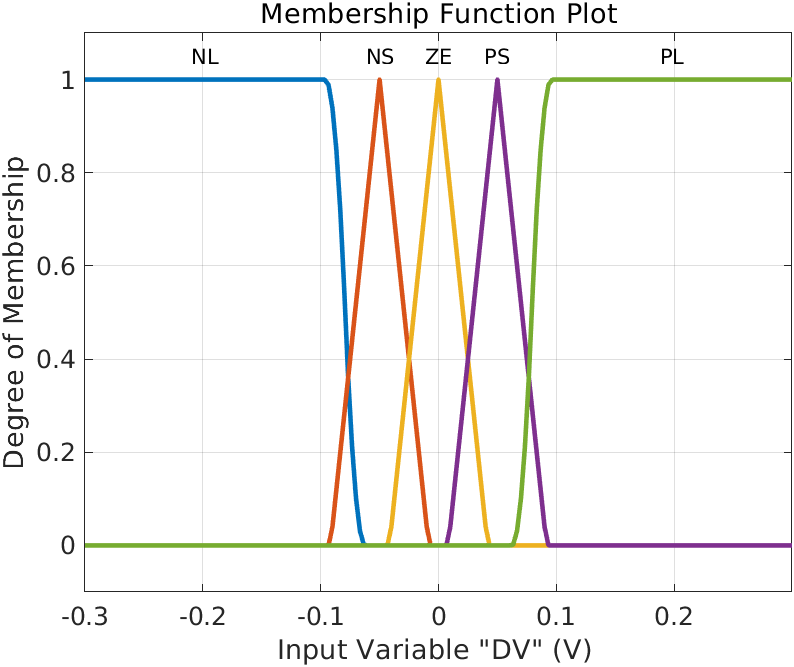
\includegraphics[width=0.8\columnwidth]{DV.png}
\caption{Membership functions for \(\Delta V\). The input is fuzzified into five linguistic variables: Negative Large (NL), Negative Small (NS), Zero (ZE), Positive Small (PS), and Positive Large (PL).}
\label{membership_deltaV}
\end{figure}

\begin{figure}[ht]
\centering
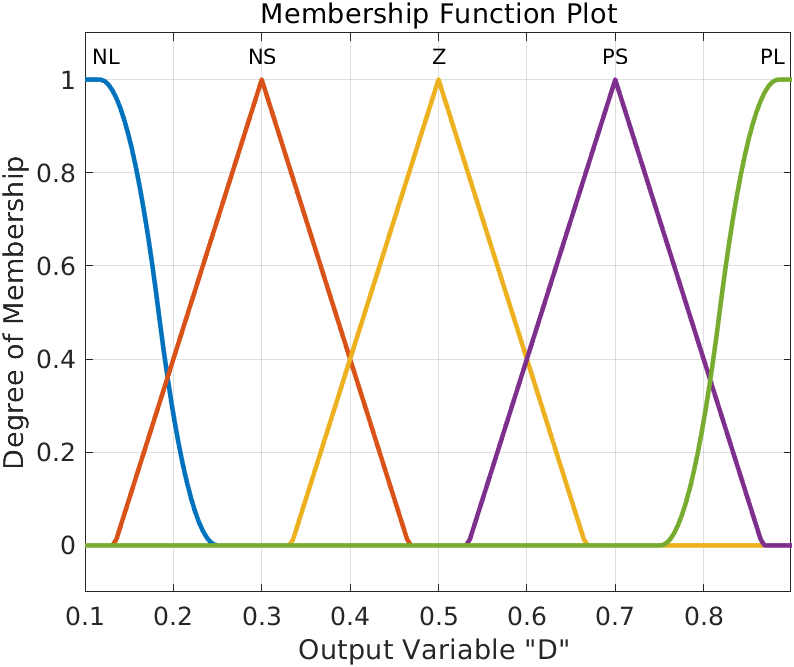
\includegraphics[width=0.75\columnwidth]{D.png}
\caption{Membership functions for the output. The control action is represented using five linguistic variables: Negative Large (NL), Negative Small (NS), Zero (ZE), Positive Small (PS), and Positive Large (PL).}
\label{fig7:membership_output}
\end{figure}

\subsubsection{Fuzzy Rules}
The fuzzy rules are designed to determine the appropriate control action based on the fuzzified inputs. A 5x5 rule table is used to map the combinations of \(\Delta P\) and \(\Delta V\) to the output. The complete rule table is at Table \ref{tab:fuzzy_rules}.

\renewcommand{\arraystretch}{1.25} 

\begin{table}[ht]
\centering
\caption{5x5 Fuzzy rule table for the FLC.}
\label{tab:fuzzy_rules}
\begin{tabular}{|c|c|c|c|c|c|}
\hline
\(\Delta V \backslash \Delta P\) & NL & NS & ZE & PS & PL \\ \hline
NL & NL & NL & NS & PS & PL \\ \hline
NS & NL & NS & NS & PS & PS \\ \hline
ZE & Z & Z & Z & Z & Z \\ \hline
PS & PL & PS & Z & NS & NS \\ \hline
PL & PL & PS & Z & NS & NL \\ \hline
\end{tabular}
\end{table}

These rules ensure that the FLC dynamically adjusts the duty cycle to track the MPP under varying conditions. For example:
\begin{itemize}
    \item If \(\Delta P\) is \textit{Negative Large (NL)} and \(\Delta V\) is \textit{Negative Large (NL)}, then the output is \textit{Negative Large (NL)}.
    \item If \(\Delta P\) is \textit{Positive Small (PS)} and \(\Delta V\) is \textit{Zero (Z)}, then the output is \textit{Positive Small (PS)}.
    \item If \(\Delta P\) is \textit{Zero (Z)} and \(\Delta V\) is \textit{Zero (Z)}, then the output is \textit{Zero (Z)}.
\end{itemize}

\begin{figure}[h]
\centering
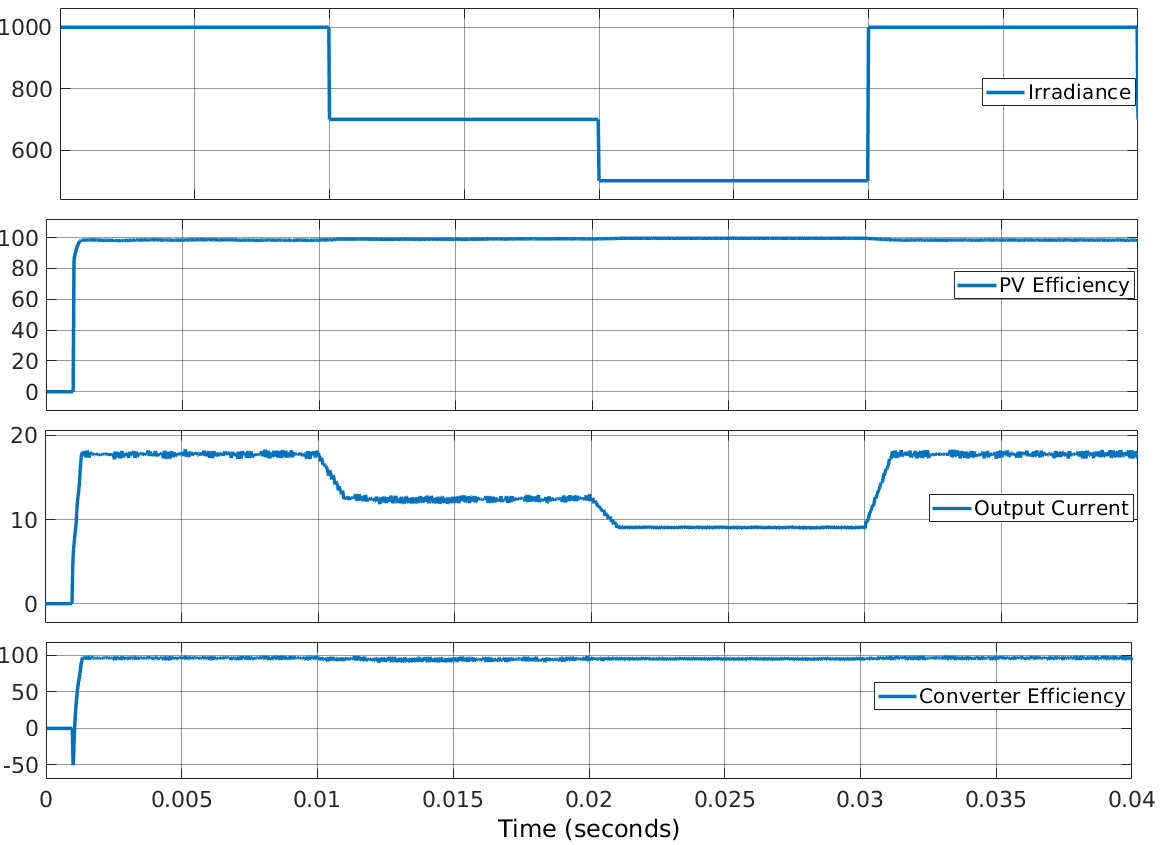
\includegraphics[width=0.95\columnwidth]{last_sim2.png}
\caption{Transient simulation results showing the system's response to dynamically changing solar irradiation. The duty cycle is dynamically adjusted to maintain the MPP, ensuring stable and efficient operation under varying conditions.}
\label{fig8:transient_simulation}
\end{figure}

\section{Simulation Results}
The performance of the proposed Fuzzy Logic-based Maximum Power Point Tracking (MPPT) system is rigorously evaluated through comprehensive simulations under dynamically changing solar irradiation conditions. The system is specifically designed to maintain stable operation and accurately track the maximum power point (MPP) even in the presence of significant variations in irradiation levels. This section presents detailed transient simulation results, highlighting the system's robustness and adaptability to fluctuating environmental conditions.

To assess the system's dynamic response, transient simulations are conducted under varying solar irradiation conditions. The irradiation level is systematically varied from 1000 W/m\(^2\) to 500 W/m\(^2\) and then back to 1000 W/m\(^2\), simulating real-world scenarios such as partial shading, cloud cover, or changes in weather. The results illustrate that the system effectively adjusts the duty cycle in real-time to maintain the MPP, ensuring optimal power transfer from the PV panel to the battery. The Fuzzy Logic Controller (FLC) demonstrates its ability to handle nonlinearities and uncertainties, providing a stable and efficient response to dynamic changes in irradiation.

The simulation result given by Figure \ref{fig8:transient_simulation} underscores the effectiveness and robustness of the proposed Fuzzy Logic-based MPPT system. The system not only tracks the MPP with high accuracy but also adapts seamlessly to sudden changes in solar irradiation. This adaptability is critical for real-world applications, where environmental conditions can vary rapidly and unpredictably. The ability to maintain stable operation under such conditions highlights the practical viability of the proposed system for use in photovoltaic battery charging applications.


\section{Conclusion}
In this paper, we presented the modeling of a Fuzzy Logic-based Maximum Power Point Tracking (MPPT) system for photovoltaic (PV) battery chargers, integrating an advanced buck converter model within a Simulink simulation framework. 
This is achieved using a buck converter model with synchronous switching, incorporating both high-side and low-side switches along with the corresponding control signaling. This approach provides a more precise representation of switching losses and non-overlapping losses.
The system is validated through comprehensive Simulink simulations under dynamically changing solar irradiation conditions, incorporating efficiency analysis, charge current evaluation, and transient response assessment. 

The simulations demonstrate a peak output current of 17.5A and a peak power efficiency of 97.5\% using the 6MN6A280 panel, selected for this application. The results highlight the benefits of integrating a refined buck converter model with fuzzy logic-based MPPT, making the approach highly suitable for PV battery charging applications in renewable energy systems. Future work will focus on developing more detailed models and transitioning towards an integrated circuit implementation of the charger system to further optimize efficiency and performance.


\section*{Acknowledgements}
This work is supported by Atek Midas, Inc., and Bogazici University.

\bibliography{references}

\end{document}